\section{Evaluation}\label{sec:eval}

\begin{figure}
  \centering
  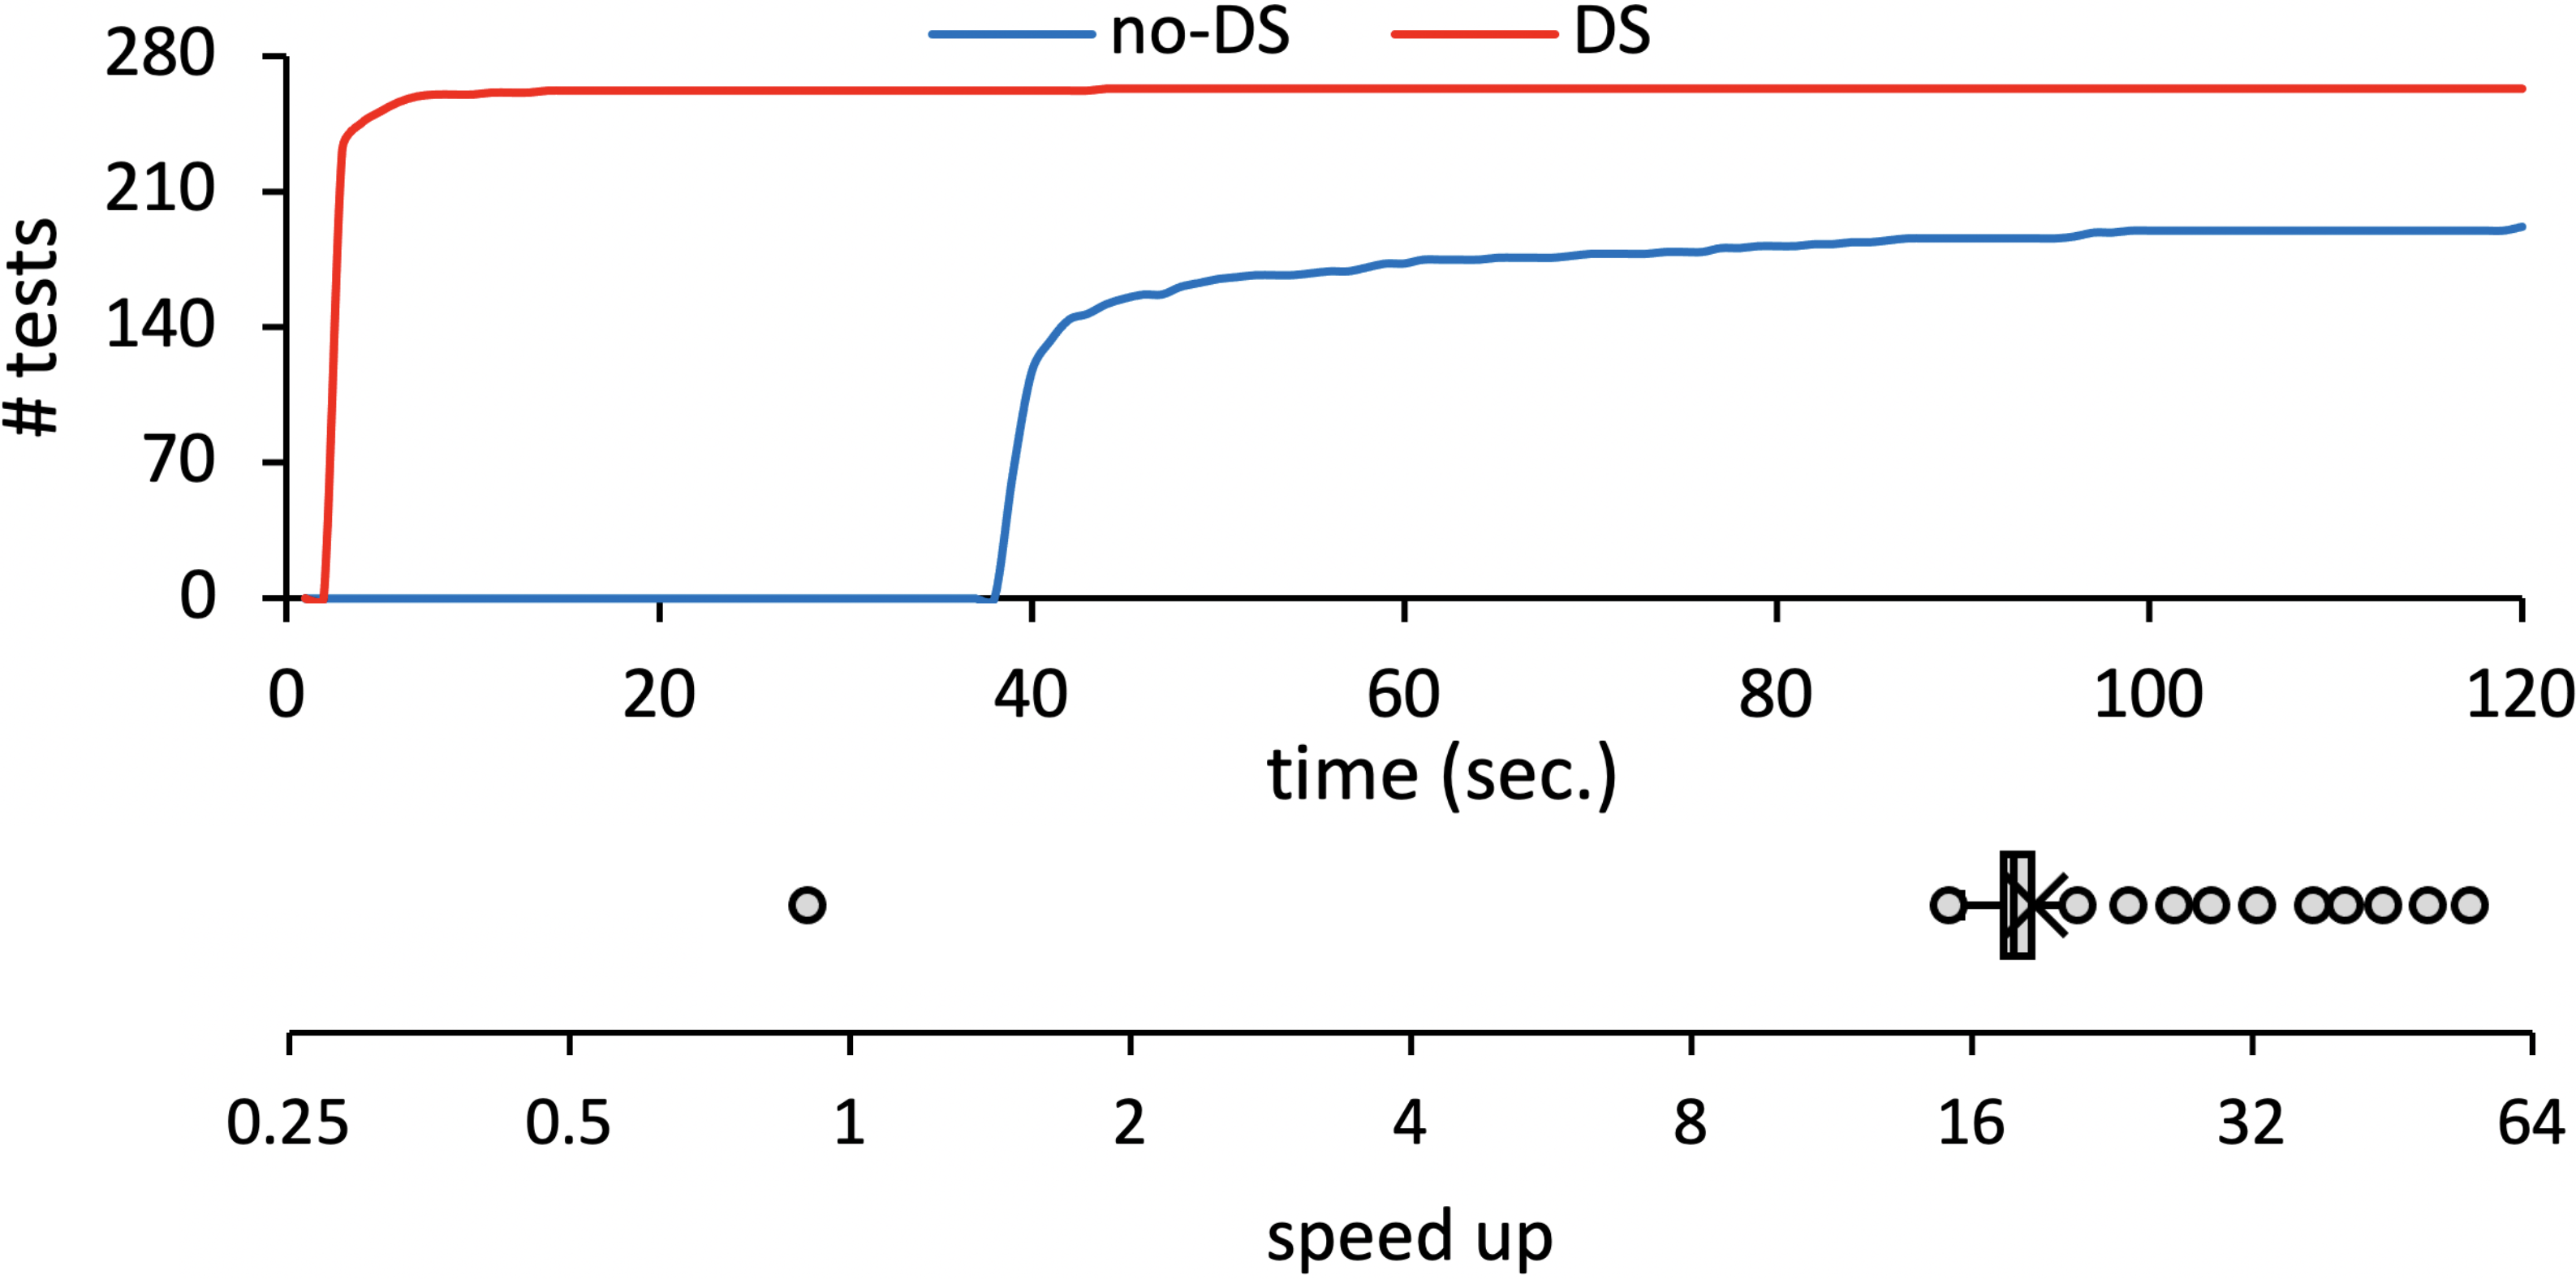
\includegraphics[width=\linewidth]{img/conc-analysis-time}
  \vspace*{-1.5em}
  \caption{Analysis time for Lodash 4 \textit{original} tests without (no-DS)
  and with (DS) the dynamic shortcut within 5 minutes.}
  \label{fig:conc-analysis-time}
  \vspace*{-1.5em}
\end{figure}

We evaluated our tool based on the following research questions:
\begin{itemize}
  \item \textbf{RQ1) Analysis Speed-up:} How much analysis time is reduced by
    adding dynamic shortcut to static analysis?
  \item \textbf{RQ2) Precision Improvement:} How much analysis precision is
    improved by replacing the manual modeling with dynamic shortcut?
  \item \textbf{RQ3) Opaque Function Coverage:} How many opaque functions are
    covered by dynamic shortcut without using manual modeling?
\end{itemize}
We targeted the official 306 tests of Lodash 4
(v.4.17.20)\footnote{https://github.com/lodash/lodash/blob/4.17.20/test/test.js}
used in motivating examples (Section~\ref{sec:motivation}).  The most recent
papers for JavaScript static analysis techniques~\cite{value-refinement,
value-partitioning} also evaluated their techniques based on them.
Among them, we filtered out \inred{37} tests including JavaScript language
features SAFE does not support, such as dynamic code generation using
\jscode{Function}, getter/setter, and browser specific features
(e.g. $\jscode{__proto__}$).  Thus, we only targeted \inred{269} out of 306
tests for the evaluation.  We performed our experiments on an Ubuntu machine
equipped with 4.2GHz Quad-Core Intel Core i7 and 64GB of RAM.


\subsection{Analysis Speed-up}

\begin{figure}
  \centering
  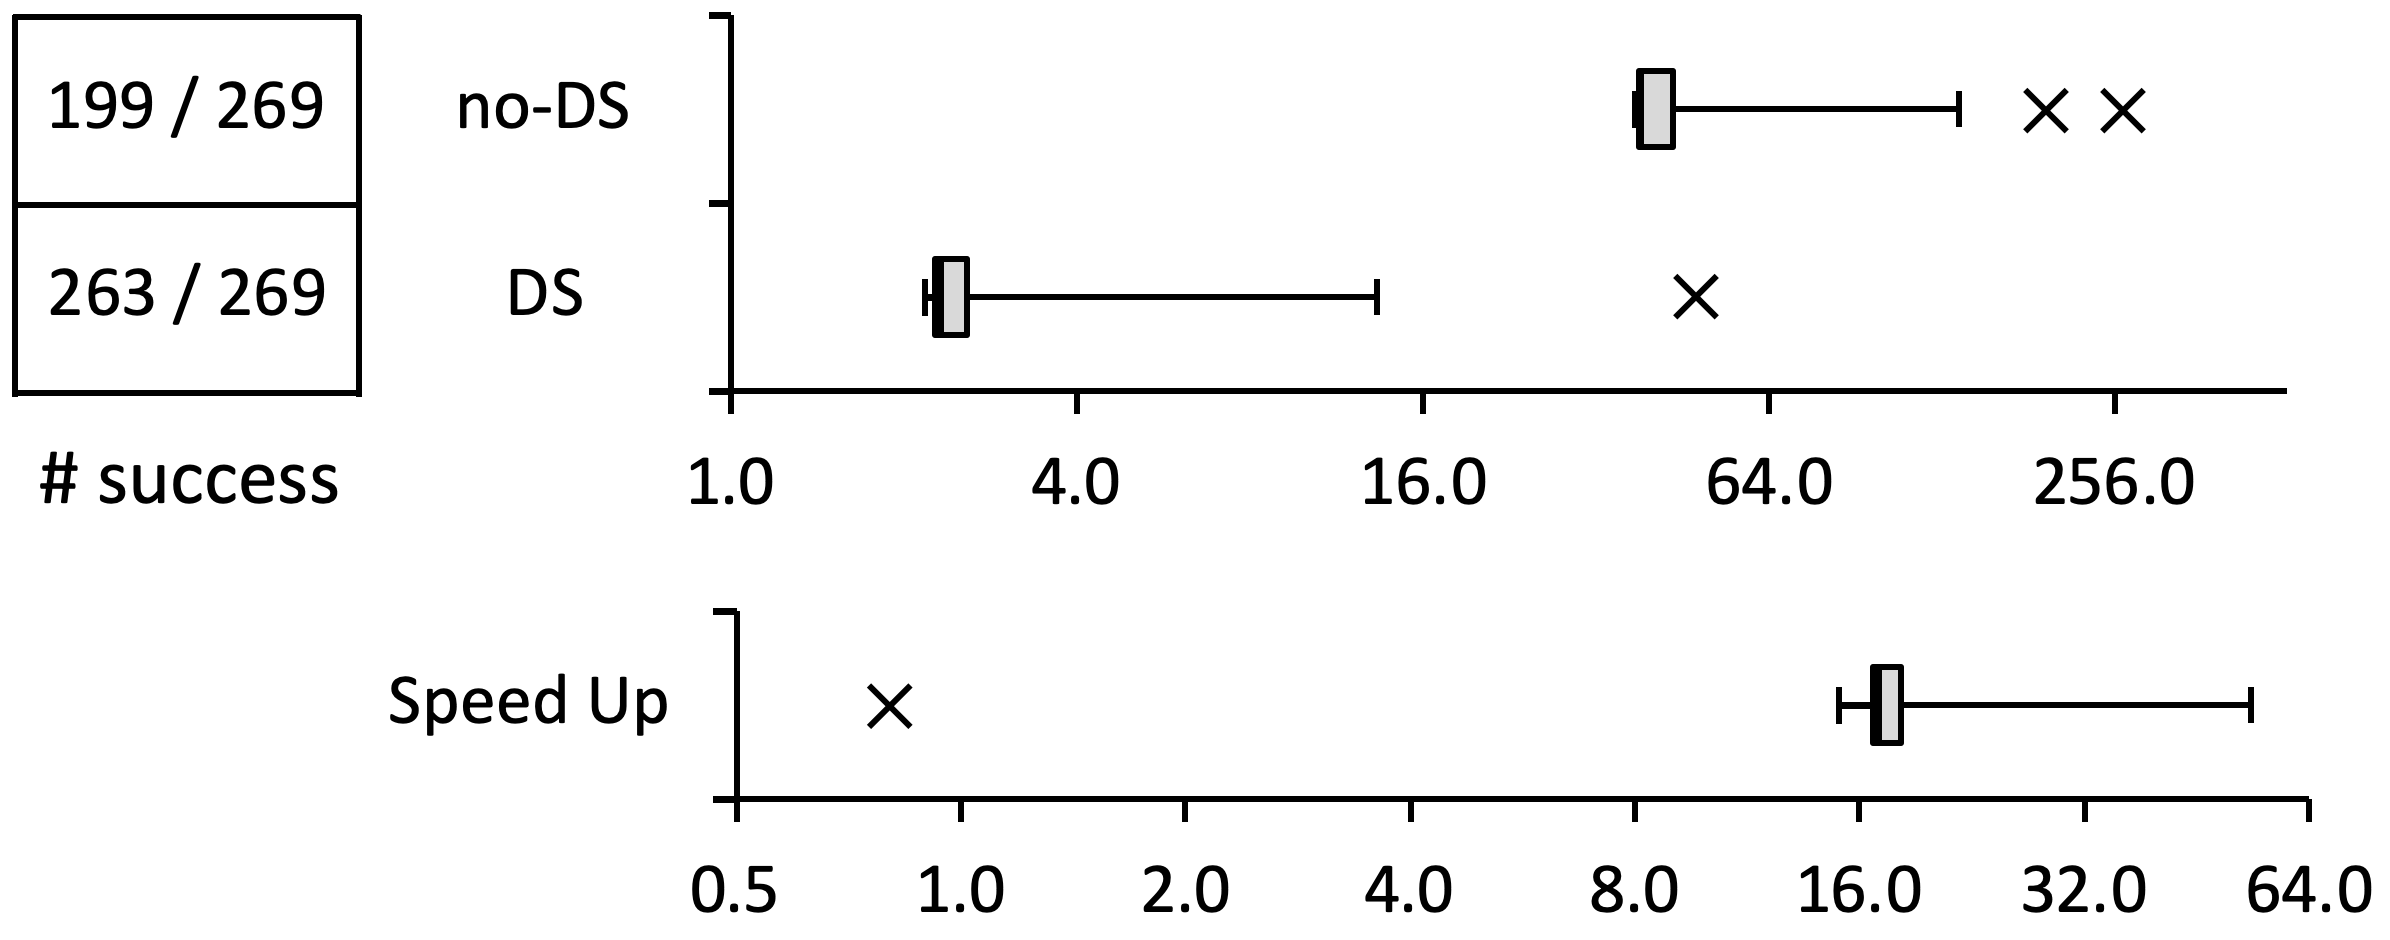
\includegraphics[width=\linewidth]{img/abs-analysis-time}
  \vspace*{-1.5em}
  \caption{Analysis time for Lodash 4 \textit{abstracted} tests without (no-DS)
  and with (DS) the dynamic shortcut within 5 minutes.}
  \label{fig:abs-analysis-time}
  \vspace*{-1.5em}
\end{figure}

To evaluate the effectiveness of the dynamic shortcut, we performed static
analysis for \inred{269} Lodash 4 tests with and without dynamic shortcut.
Figure~\ref{fig:conc-analysis-time} depicts the box plot chart for their
analysis time and for speed up after applying the dynamic shortcut in a
logarithmic scale.  While the base analysis (no-DS) finished \inred{199} out of
\inred{269} tests within 5 minutes, our tool finished all tests with the dynamic
shortcut (DS).  For \inred{199} tests analyzable by both analyses, the analysis
took \inred{168.4} seconds and \inred{12.2} seconds on average without dynamic
shortcut (no-DS) and with dynamic shortcut (DS), and the dynamic shortcut
accelerates \inred{20.16}\textsf{x} the static analysis on average.  Only for
one test using $\jscode{_.sample}$ (a Lodash 4 library that randomly samples a
value from a given array), the static analysis using dynamic shortcut had
\inred{0.81}\textsf{x} speed of the base analysis because of the frequent use of
dynamic shortcut (\inred{24} times).

Unfortunately, since most of Lodash 4 tests use concrete values instead of
non-deterministic user inputs, they could be analyzed via a few number of
dynamic shortcut.  In fact, among \inred{269} tests, \inred{262} tests analyzed
via a single usage of dynamic shortcut without using abstract semantics.
However, the arguments of library functions might include non-deterministic user
inputs in the real-world JavaScript programs.  Thus, we modified Lodash 4
official tests with abstract values to mimic the use patterns of library
functions.  We randomly selected literals and replace subset of them to their
corresponding typed abstract values.  For example, if we pick a numerical
literal \jscode{42}, we modified it to the abstract numeric value
$\top_{\code{num}}$, which represents the all numerical values.  In the
remaining section, we evaluated our tool based on the randomly abstracted tests
of Lodash 4.

For abstracted tests, the dynamic shortcut successfully accelerates the static
analysis.  Figure~\ref{fig:abs-analysis-time} shows the analysis time for the
abstracted tests in a logarithmic scale.  Among \inred{269} abstracted tests,
the base analysis (no-DS) finished \inred{82} tests within 5 minutes.  On the
other hand, the analysis using dynamic shortcut (DS) finished \inred{219} tests.
For \inred{82} tests analyzable by both analyses, the analyses took
\inred{168.4} seconds and \inred{12.2} seconds on average without dynamic
shortcut (no-DS) and with dynamic shortcut (DS), and the dynamic shortcut
accelerates \inred{20.16}\textsf{x} the static analysis on average.

\begin{figure}
  \centering
  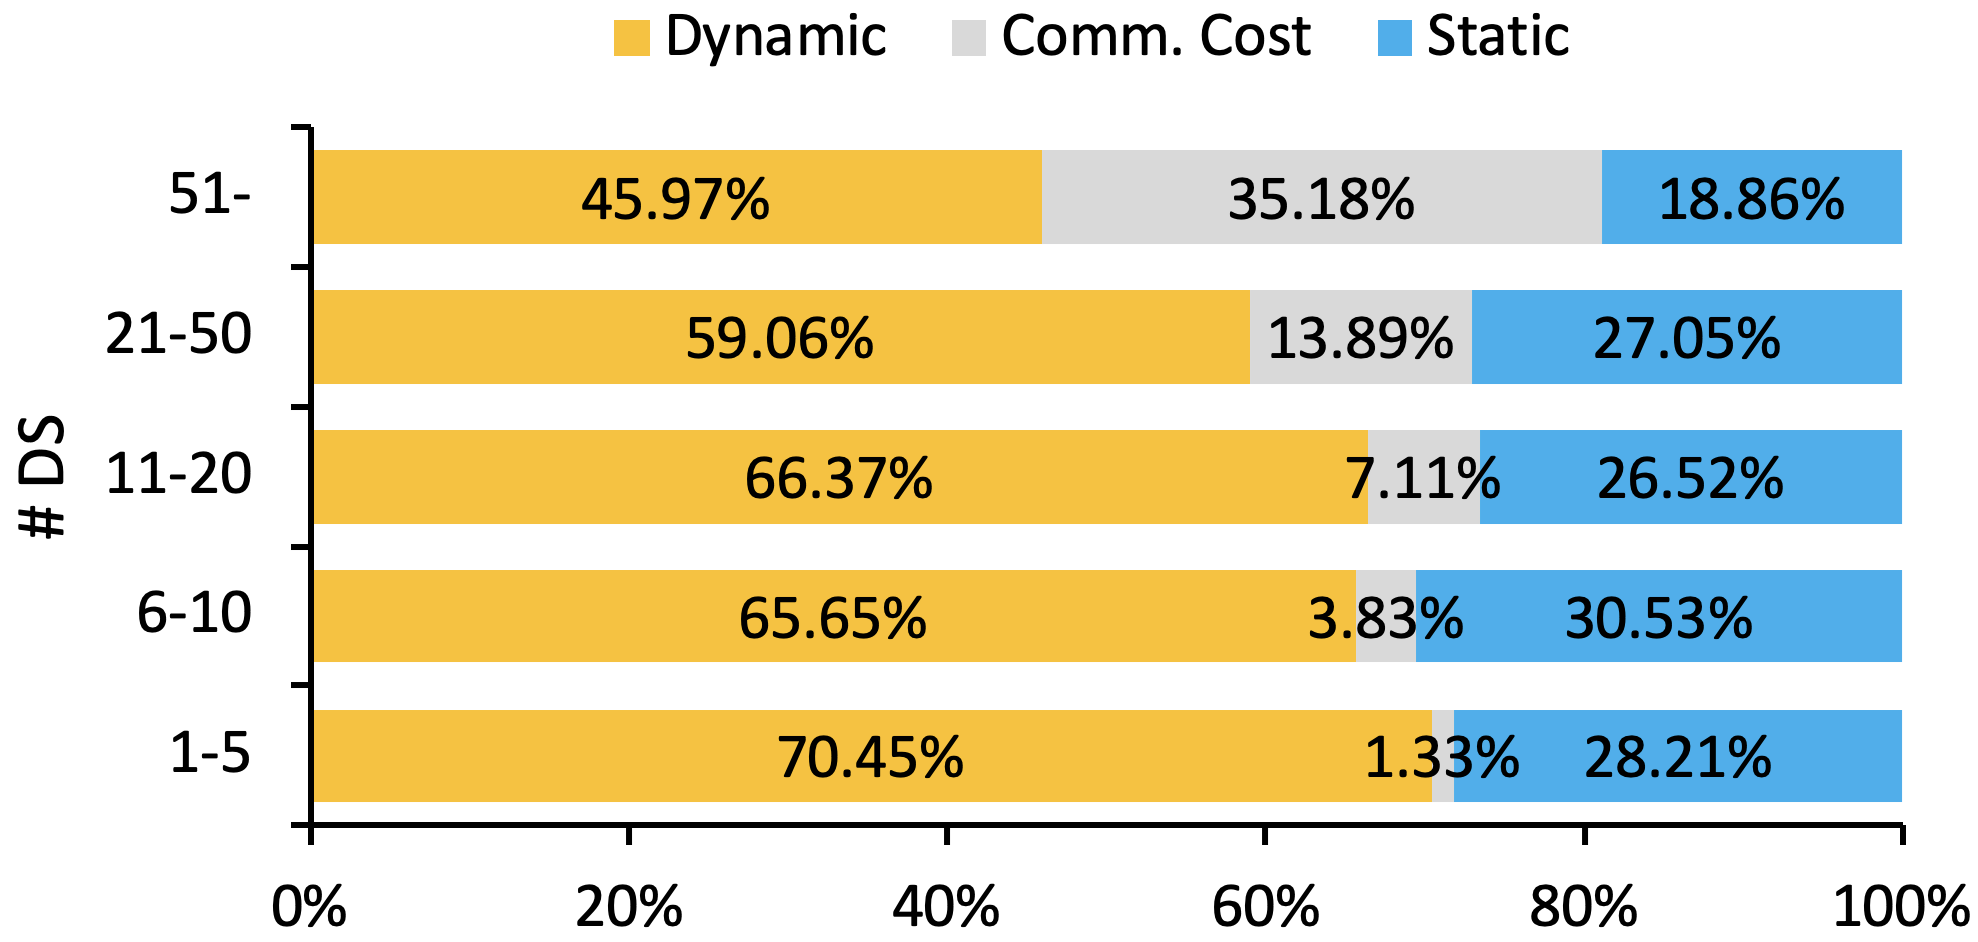
\includegraphics[width=\linewidth]{img/abs-analysis-ratio}
  \vspace*{-1.5em}
  \caption{Time ratio of the finished analysis with dynamic shortcut for
  \inred{219} Lodash 4 \textit{abstracted} tests.}
  \label{fig:abs-analysis-ratio}
  \vspace*{-1.5em}
\end{figure}

For \inred{219} abstracted tests successfully analyzed with the dynamic
shortcut, communication costs between static and dynamic analysis grew
relatively to the number of dynamic shortcuts.  To communicate with the
dynamic analyzer, the static analysis should dump the current abstract state,
send it to the dynamic analyzer, receive the result from the dynamic analysis,
and apply the given update information to the abstract state.  Thus, the
communication costs will increase dependent on the number of dynamic shortcuts.
Figure~\ref{fig:abs-analysis-ratio} shows the time ratio of dynamic and static
analysis parts with communication costs in total analysis time.  On average, the
dynamic analysis occupied \inred{63.30}\%, communication \inred{9.52}\%, and
static analysis \inred{27.17}\% in total analysis time.  If the dynamic
shortcuts are performed less than 10 times, the ratio of communication in total
analysis time is \inred{9.50\%} on average.  The more dynamic shortcuts
performed, the more communication cost is required.  When the number is
between 41 and 50, the ratio of average communication cost is rised to
\inred{10.65\%} in the total analysis time.


\subsection{Precision Improvement}

To evaluate the precision improvement of dynamic shortcut, we used two different
metrics to measure the precision of the analysis results: 1) the number of false
alarms for assertions in tests and 2) the number of branch covered by analysis.
Figure~\ref{fig:precision} depicts the comparison of analysis precision without
(no-DS) and with (DS) dynamic shortcut using two different metrics.

Lodash 4 official tests check the assertions based on
QUnit\footnote{https://qunitjs.com/}, which is a powerful, easy-to-use
JavaScript testing framework.  Since all assertions in each test are passed in
the concrete execution, any assertion failures during static analysis should be
false alarms.  Although we analyzed \textit{abstracted} Lodash 4 tests, the
number of assertion failures during static anlysis could be a metric of
imprecision of the analysis.  Figure~\ref{fig:precision-fail} shows the number
of assertion failures in each test analyzable by both analysis with and
without dynamic shortcut.  The $x$- and $y$-axis denote the analysis without
(no-DS) and with (DS) dynamic shortcut and each $\times$ mark denotes each test.
The top and bottom dotted lines denote the worst and best precision improvement,
and the middle solid line denotes the average improvement.  Thus, dynamic
shortcut reduces assertion failures to at least \inred{1.00}\textsc{x}, at most
\inred{0.54}\textsc{x}, and \inred{0.92}x on average.

Another metric to measure the precision of static analysis is the number of
branches covered during analysis.  If the static analysis is sound, the more
precise analysis covers the less number of branches.  In the similar way with
the number of assertion failures, Figure~\ref{fig:precision-branch} depicts the
the comparison of the number of branches during static analysis without (no-DS)
and with (DS) dynamic shortcut.  In the view point of the branch coverage,
dynamic shortcut successfully cut down the number of covered branches at least
\inred{0.81}\textsc{x}, at most \inred{0.51}\textsc{x}, and
\inred{0.68}\textsc{x} on average.

\begin{figure}
  \centering
  \begin{subfigure}[t]{0.48\textwidth}
    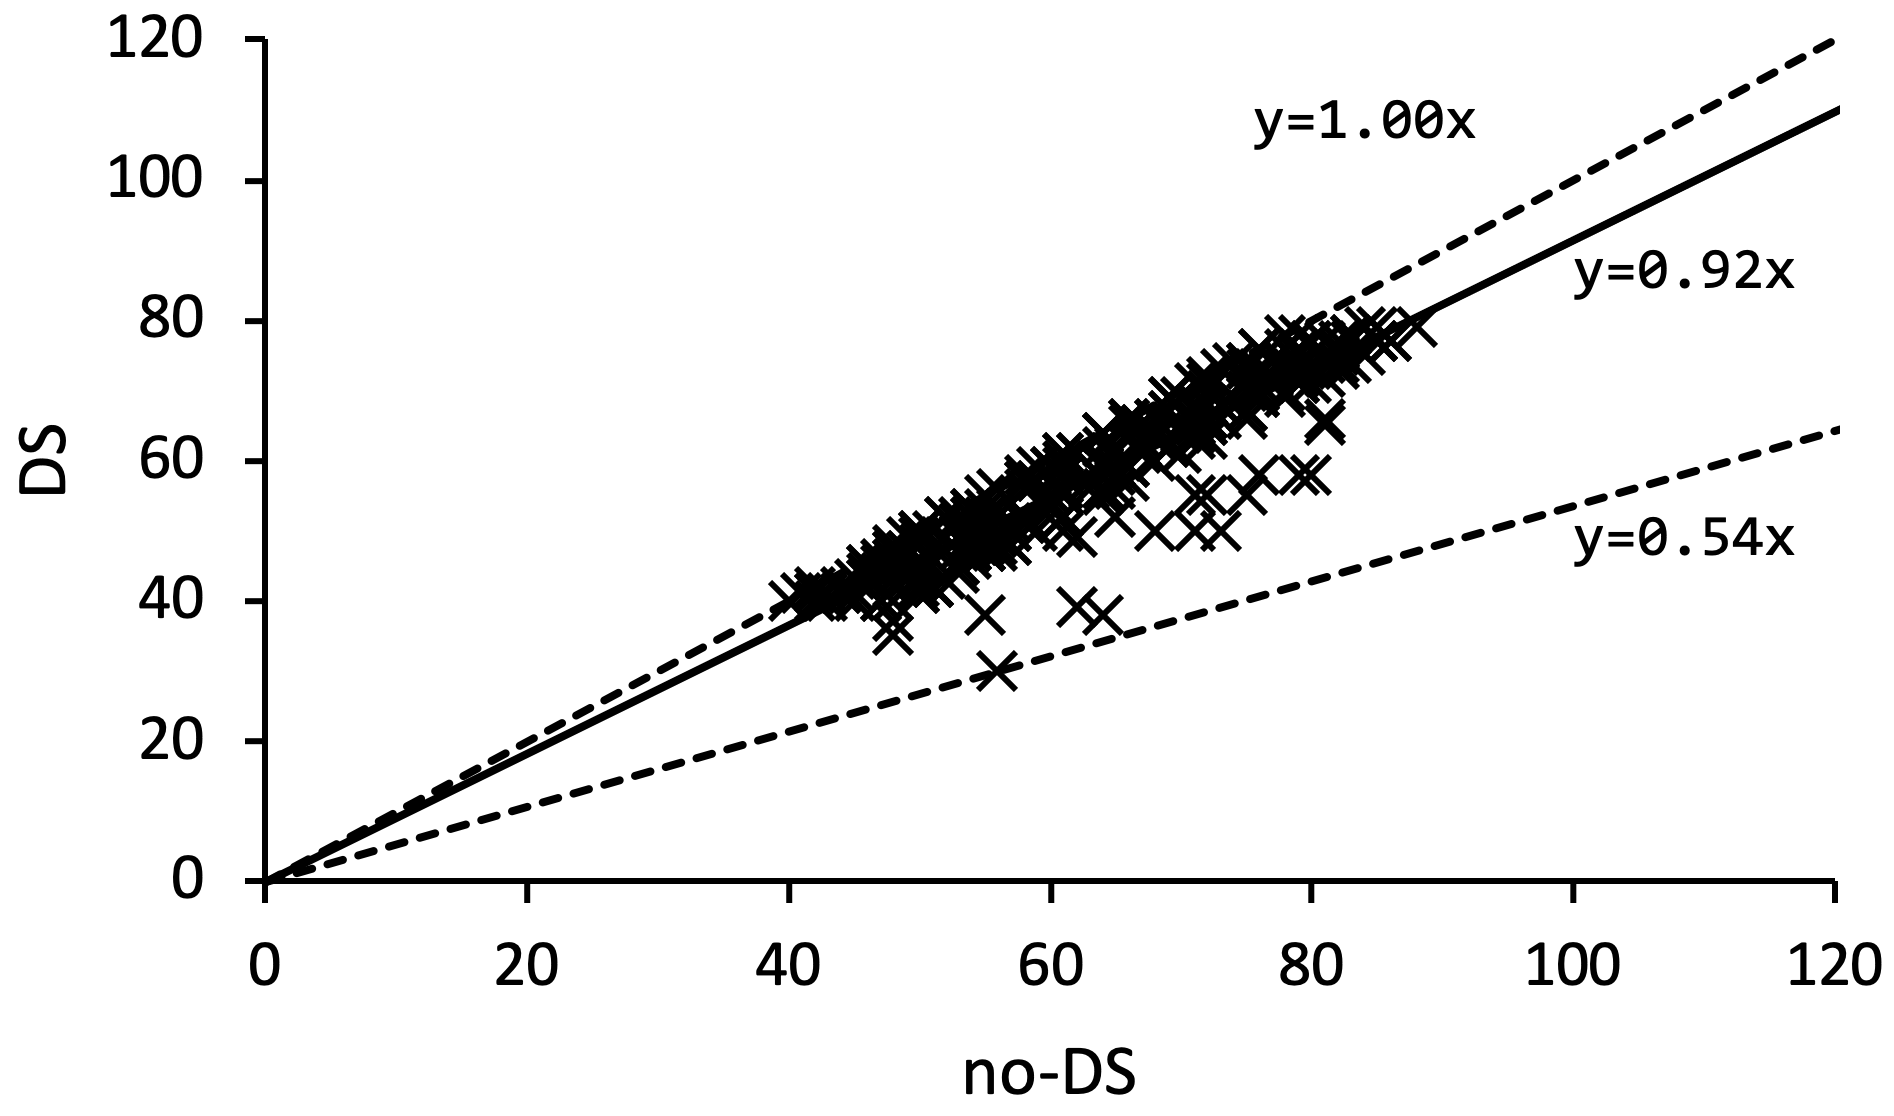
\includegraphics[width=\linewidth]{img/precision-fail}
    \vspace*{-1.5em}
    \caption{\# Failed Assertions.}
    \label{fig:precision-fail}
  \end{subfigure}
  \begin{subfigure}[t]{0.48\textwidth}
    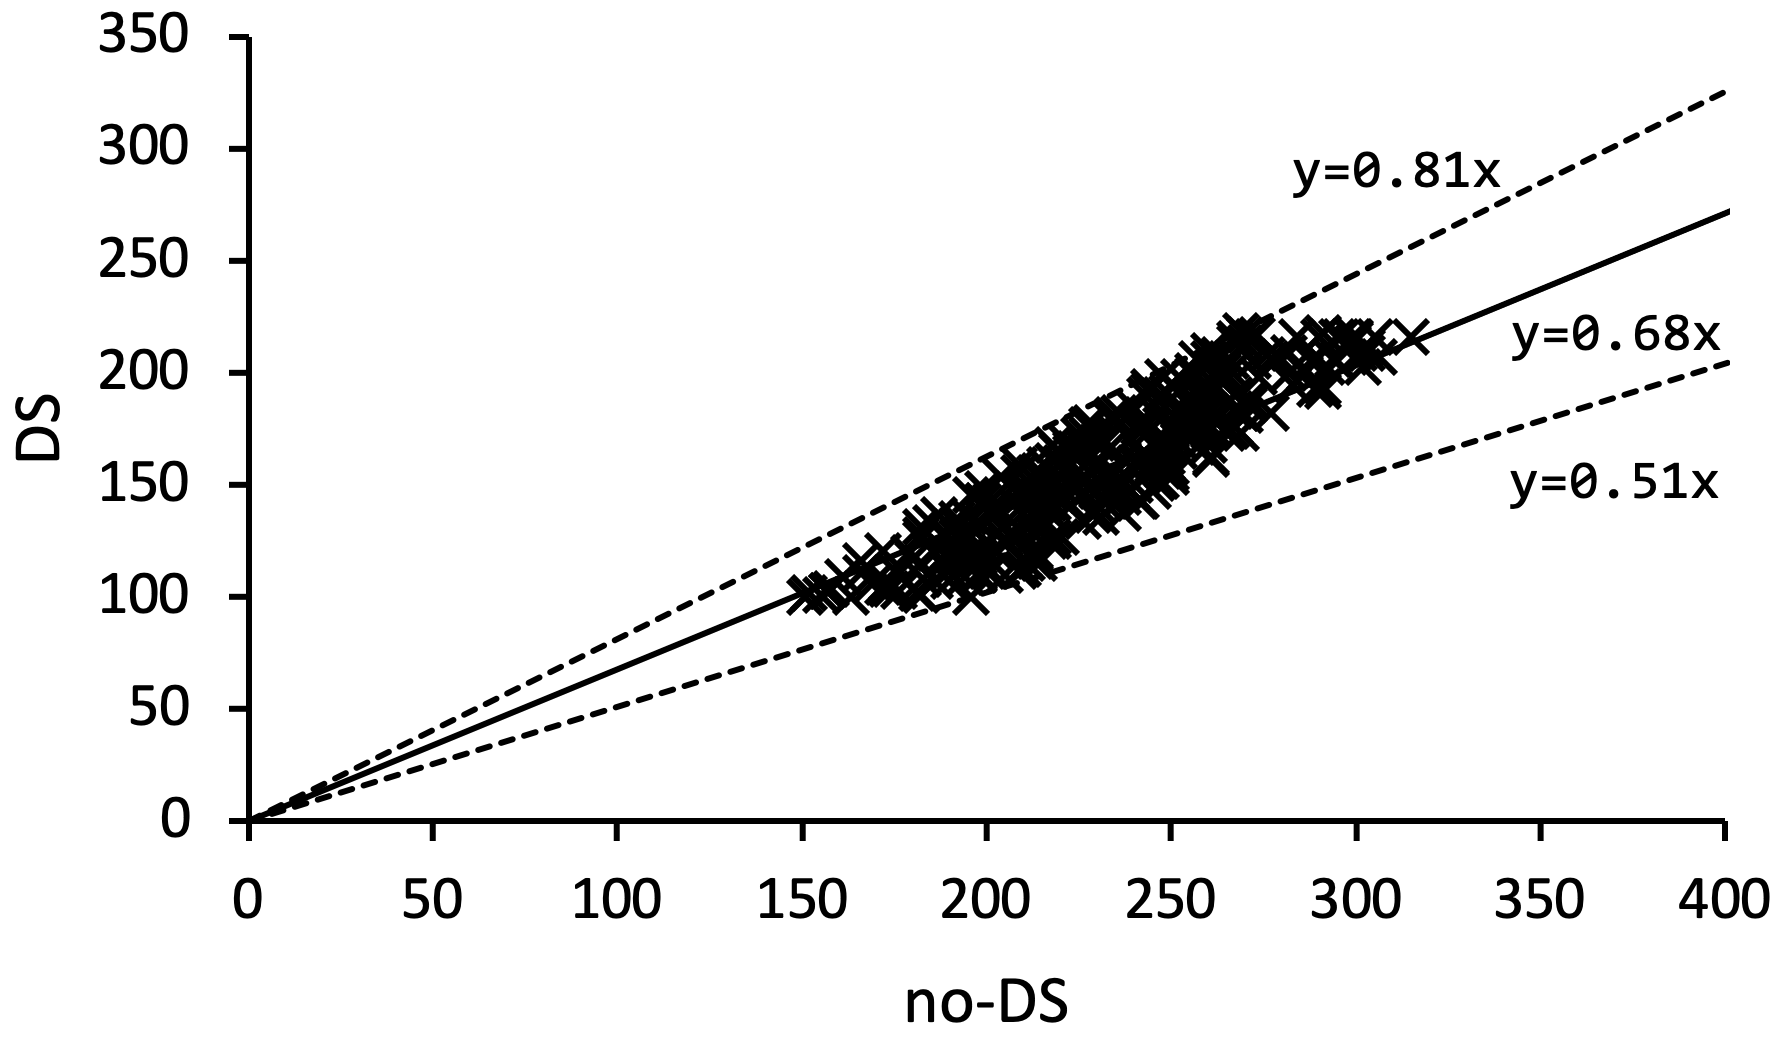
\includegraphics[width=\linewidth]{img/precision-branch}
    \vspace*{-1.5em}
    \caption{\# Covered Branches.}
    \label{fig:precision-branch}
  \end{subfigure}
  \vspace*{-1em}
  \caption{The comparison of analysis precision without (no-DS) and with (DS)
  dynamic shortcut for \inred{82} \textit{abstracted} tests analyzable by both
  analyses}
  \label{fig:precision}
  \vspace*{-1.5em}
\end{figure}


\subsection{Opaque Function Coverage}

\begin{table*}
  \centering
  \scriptsize
  \[
    \begin{array}{c|l|@{~}r@{~}c@{~}r@{~}r@{~}?c|l|@{~}r@{~}c@{~}r@{~}r@{~}?c|l|@{~}r@{~}c@{~}r@{~}r@{~}}
      \myhead
      \mysucc{2}{Boolean}   {Boolean}         {214}{214}{100} & \mydata{1}{}            {new Object}        {214}{214}{100} & \mymult{2}{Number}      {valueOf}       {214}{214}{100} \mylineff
      \mydata{1}{}          {new Boolean}     {214}{214}{100} & \mydata{1}{}            {getPrototypeOf}    {214}{214}{100} & \myname{1}{.prototype}                                  \mylinetft
      \mydata{1}{Array}     {isArray}         {214}{214}{100} & \mydata{1}{}            {create}            {214}{214}{100} & \mymult{2}{RegExp}      {toString}      {214}{214}{100} \mylinetf
      \mydata{1}{}          {toString}        {214}{214}{100} & \mydata{1}{Object}      {preventExtensions} {214}{214}{100} & \myname{1}{.prototype}                                  \mylinefft
      \mydata{1}{}          {toLocaleString}  {214}{214}{ 90} & \mydata{1}{}            {isFrozen}          {214}{214}{100} & \mydata{2}{String}      {String}        {214}{214}{100} \mylinefff
      \mydata{1}{}          {concat}          {214}{214}{100} & \mydata{1}{}            {isExtensible}      {214}{214}{100} & \mydata{1}{}            {fromCharCode}  {214}{214}{100} \mylinefft
      \mydata{1}{}          {join}            {214}{214}{100} & \mydata{1}{}            {keys}              {214}{214}{100} & \mydata{1}{}            {charAt}        {214}{214}{100} \mylineftf
      \mysucc{1}{Array}     {pop}             {214}{214}{100} & \mydata{1}{Object}      {valueOf}           {214}{214}{100} & \mydata{1}{}            {charCodeAt}    {214}{214}{100} \mylinefff
      \mydata{1}{.prototype}{push}            {214}{214}{100} & \mydata{1}{.prototype}  {isPrototypeOf}     {214}{214}{100} & \mydata{1}{}            {indexOf}       {214}{214}{100} \mylineftf
      \mydata{1}{}          {slice}           {214}{214}{100} & \mydata{1}{}            {acos}              {214}{214}{100} & \mysucc{1}{}            {match}         {214}{214}{100} \mylinefff
      \mydata{1}{}          {splice}          {214}{214}{100} & \mysucc{1}{}            {atan2}             {214}{214}{100} & \mydata{1}{String}      {replace}       {214}{214}{100} \mylinefff
      \mydata{1}{}          {map}             {214}{214}{100} & \mydata{1}{}            {cos}               {214}{214}{100} & \mydata{1}{.prototype}  {splice}        {214}{214}{100} \mylinefff
      \mydata{1}{}          {reduce}          {214}{214}{100} & \mydata{1}{Math}        {exp}               {214}{214}{100} & \mydata{1}{}            {split}         {214}{214}{100} \mylinetff
      \mysucc{1}{global}    {eval}            {214}{214}{100} & \mydata{1}{}            {floor}             {214}{214}{100} & \mysucc{1}{}            {substring}     {214}{214}{100} \mylinetff
      \mydata{1}{}          {new Date}        {214}{214}{100} & \mydata{1}{}            {max}               {214}{214}{100} & \mydata{1}{}            {toLowerCase}   {214}{214}{100} \mylinefff
      \mydata{1}{Date}      {parse}           {214}{214}{100} & \mydata{1}{}            {min}               {214}{214}{100} & \mydata{1}{}            {toUpperCase}   {214}{214}{100} \mylinef
      \mydata{1}{}          {now}             {214}{214}{100}
    \end{array}
  \]
  \caption{\todo}
  \label{fig:abs-analysis-ratio}
  \vspace*{-1.5em}
\end{table*}

\todo
